\FloatBarrier
\section{Milestone III}
Now we introduce density perturbations to our baseline cosmology, and study the evolution of these perturbations. Perturbations apply to photon multipoles, baryon and dark matter density and velocity, and to the gravitational metric.

Citations: \citet{maCosmologicalPerturbationTheory1995}

\subsection{Theory}
We can derive a system of ODEs to solve in order to study perturbations. See \citet[part 3, cosmological perturbation theory]{wintherCosmologyIILecture2024} for derivation of these equations. The main equations to solve are eqs. \ref{eq:cdm_baryon_perturbations} and \ref{eq:metric_perturbations}, for matter perturbations (CDM, baryons) and perturbations of the graviational metric respectively.

\begin{equation}\label{eq:cdm_baryon_perturbations}
\boxed{
\begin{aligned}
\delta_{\rm CDM}^\prime &= \frac{ck}{\mathcal{H}} v_{\rm CDM} - 3\Phi^\prime \\
v_{\rm CDM}^\prime &= -v_{\rm CDM} -\frac{ck}{\mathcal{H}} \Psi \\
\delta_b^\prime &= \frac{ck}{\mathcal{H}}v_b -3\Phi^\prime \\
v_b^\prime &= -v_b - \frac{ck}{\mathcal{H}}\Psi + \tau^\prime R(3\Theta_1 + v_b) \\
\end{aligned}
}
\end{equation}

\begin{equation}\label{eq:metric_perturbations}
\boxed{
\begin{aligned}
\Phi^\prime &= \Psi - \frac{c^2k^2}{3\mathcal{H}^2} \Phi + \\
    &+ \frac{H_0^2}{2\mathcal{H}^2} \left[\Omega_{\rm CDM 0} a^{-1} \delta_{\rm CDM} + \Omega_{b 0} a^{-1} \delta_b + 4\Omega_{\gamma 0}a^{-2}\Theta_0\right] \\
\Psi &= -\Phi - \frac{12H_0^2}{c^2k^2a^2}\left[\Omega_{\gamma 0}\Theta_2\right] \\
\end{aligned}
}
\end{equation}

$R$ is the same as earlier, $R = \frac{4\Omega_{\gamma 0}}{3\Omega_{b 0} a}$.

However, these equations are affected by the temperature and photon hotspots in the fluid we are considering to be the universe. Photons, unlike baryons, have multipolar effects, which enter as $\Theta_\ell$. Each $\Theta_\ell$ depends on $\Theta_{\ell+1}$, which makes for an infinite set of equations to solve. Thankfully, line of sight integration as developed by (Zaldarriaga and Seljak) can solve this problem, providing an alternate means of calculating a power spectrum from the Boltzmann equations we started with. (See lecture notes citation). Line of sight integration only needs a few starting multipoles for verification, so in this project we will truncate the multipole hierarchy at around six.

Apart from photon multipoles, there are also additional effects from both neutrino multipoles and polarization of the photon fluid. These will not be treated in this project, instead see for example (something where they actually do it). But here, we treat $\mathcal{N}_\ell = 0$ and $\Theta^P_\ell = 0$.

The equations for photon multipoles to be included are eq. \ref{eq:photon_multipoles}.

\begin{equation}\label{eq:photon_multipoles}
\boxed{
\begin{aligned}
\Theta^\prime_0 &= -\frac{ck}{\mathcal{H}} \Theta_1 - \Phi^\prime \\
\Theta^\prime_1 &=  \frac{ck}{3\mathcal{H}} \Theta_0 - \frac{2ck}{3\mathcal{H}}\Theta_2
    + \frac{ck}{3\mathcal{H}}\Psi + \tau^\prime\left[\Theta_1 + \frac{1}{3}v_b\right] \\
&\begin{split}
\Theta^\prime_\ell = \frac{\ell ck}{(2\ell+1)\mathcal{H}}&\Theta_{\ell-1} - \frac{(\ell+1)ck}{(2\ell+1)\mathcal{H}} \Theta_{\ell+1} \\
    &+ \tau^\prime\left[\Theta_\ell - \frac{1}{10}\Pi \delta_{\ell,2}\right], \quad 2 \le \ell < \ell_{\textrm{max}}
    \end{split} \\
\Theta_{\ell}^\prime &= \frac{ck}{\mathcal{H}} \Theta_{\ell-1}
    - c\frac{\ell+1}{\mathcal{H}\eta(x)}\Theta_\ell + \tau^\prime\Theta_\ell, \quad \ell = \ell_{\textrm{max}}\\
\end{aligned}
}
\end{equation}

\subsection{Implementation details}
%Something about the numerical work.

\subsection{Results}
See figs. \ref{fig:milestone_3_delta_gamma_delta_b_delta_cdm}, \ref{fig:milestone_3_v_b_v_cdm}, \ref{fig:milestone_3_phi}, \ref{fig:milestone_3_phi_plus_psi}, \ref{fig:milestone_3_theta_0}, \ref{fig:milestone_3_theta_1}.

Recombination happened too late, and whatever was going on there seems to have severely interfered with these results. No time to investigate properly, though. Presumably the pipeline is fine and just needs fixes to the calculations, and then these plots would turn out as they should.

\begin{figure}[h!tbp]
\centering
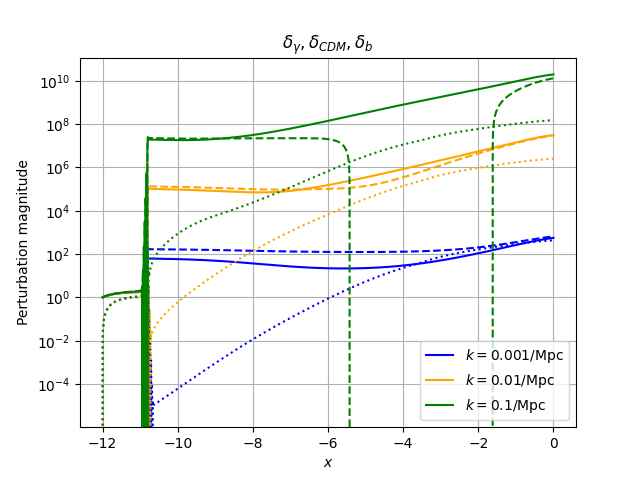
\includegraphics[width=0.4\textwidth]{../Milestone 3/Plots/delta_gamma_delta_b_delta_cdm_plot.png}
\caption{Perturbations to densities, represented by the parameter $\delta$ presented by \citet{wintherCosmologyIILecture2024}. CDM perturbations are represented by the solid line, baryon perturbations by the dashed line, and photon perturbations by the dotted line. Photon perturbations evolve mostly unaffected by the matter perturbations, which is good. Baryons might be oscillating away from the dark matter (due to baryon dragging) as expected, but fall off the scale of the plot. Early time development is completely messed up. Different scales might be entering evolution at different times as expected, but this is hard to tell.}
\label{fig:milestone_3_delta_gamma_delta_b_delta_cdm}
\end{figure}

\begin{figure}[h!tbp]
\centering
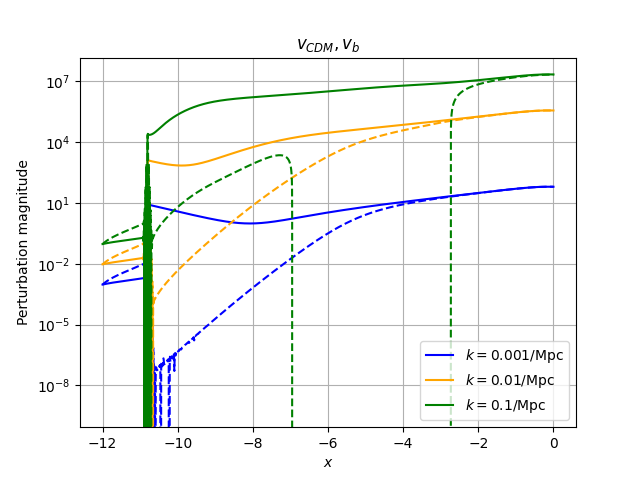
\includegraphics[width=0.4\textwidth]{../Milestone 3/Plots/v_b_v_cdm_plot.png}
\caption{Similar to fig. \ref{fig:milestone_3_delta_gamma_delta_b_delta_cdm}, but for perturbed average velocities of the respective quantities. Early times are completely messed up.}
\label{fig:milestone_3_v_b_v_cdm}
\end{figure}

\begin{figure}[h!tbp]
\centering
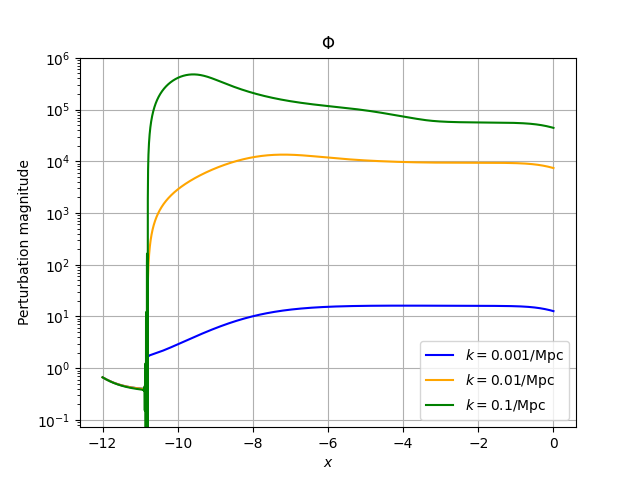
\includegraphics[width=0.4\textwidth]{../Milestone 3/Plots/phi_plot.png}
\caption{Perturbations to the graviational metric, component $\Phi$. The scale dependency is wrong, modes that enter early should fall off to zero much more aggressively. Perturbations should start around the same size and stay relatively constant until re-entering the horizon. We do not observe the change in evolution as the universe starts to become dominated by dark energy at the very end.}
\label{fig:milestone_3_phi}
\end{figure}

\begin{figure}[h!tbp]
\centering
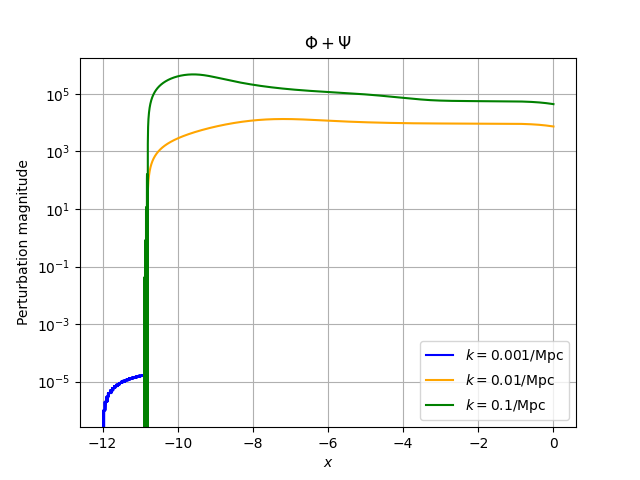
\includegraphics[width=0.4\textwidth]{../Milestone 3/Plots/phi_plus_psi_plot.png}
\caption{Combined perturbations to the graviational metric. Same problems as fig. \ref{fig:milestone_3_phi}.}
\label{fig:milestone_3_phi_plus_psi}
\end{figure}

\begin{figure}[h!tbp]
\centering
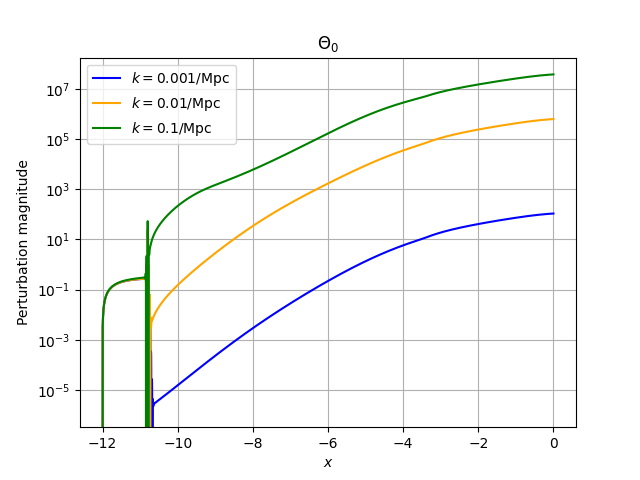
\includegraphics[width=0.4\textwidth]{../Milestone 3/Plots/theta_0_plot.png}
\caption{The evolution of the photon monopole. Modes should be re-entering at different times to start a significant dampened oscillation, but the plot is messed up.}
\label{fig:milestone_3_theta_0}
\end{figure}

\begin{figure}[h!tbp]
\centering
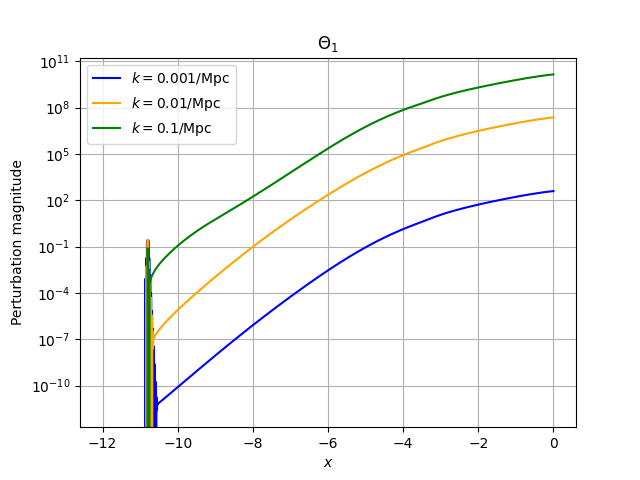
\includegraphics[width=0.4\textwidth]{../Milestone 3/Plots/theta_1_plot.png}
\caption{Evolution of the photon dipole. Same problems as fig. \ref{fig:milestone_3_theta_0}.}
\label{fig:milestone_3_theta_1}
\end{figure}
